\chapter{はじめに}
本論文では,大学に関する記事から文書毎のベクトルを生成することによって各大学毎の特色をデータ化し,潜在的な関係性を可視化する研究について記述する.

まず,本研究をおこなう背景となった事柄について述べる.
次に,研究目的の詳細について述べ,最後に次章以降の本論文の構成について概略を述べる.

\section{背景}
近年,大学進学という選択肢は高校生にとって,一般的な選択肢として受け入れられるようになった.
図 \ref{fig:univ_continuance_rate}に文部科学省による過去10年間の大学・短大進学率と,大学(学部)進学率の推移の資料\cite{univContinuanceRate}を示す.  
直近3年間の推移は比較的横ばい傾向にあるが,高校卒業後の進路に関して50\%近い学生が大学へ進学している.

さらに,2020年4月から高等教育の修学支援制度\cite{Shingakusyusienseido}が施行される.
この新制度では,学生個人に対する要件と支援対象者の所得に関する要件を満たした場合に,授業料などを減免するか給付型の奨学金を支給する.
その対象となる学校種は大学,短期大学,高等専門学校,専門学校である.
% 前提として,少子化が進んでいるために全体の大学進学者数は減少傾向にあるが,この制度の施行により,大学・専門学校進学率は今後増加すると考えられる.
少子化の発展のため大学進学者は減少すると予想される一方で,この制度の影響によって,大学への進学率そのものは増加すると考えられる.
\begin{figure}[H]
\centering
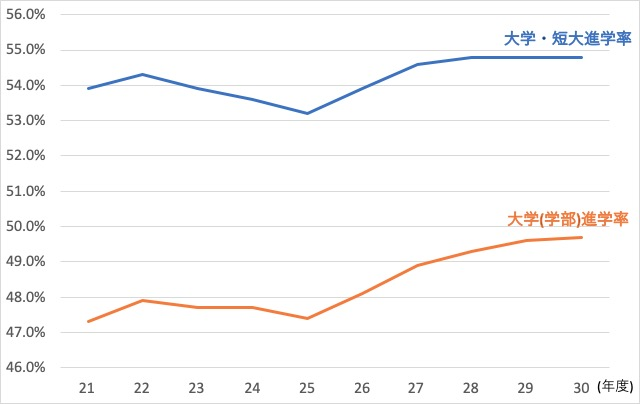
\includegraphics[scale=0.63]{images/univ_continuance_rate.jpg}
\caption{過去10年間の大学進学率推移}
\label{fig:univ_continuance_rate}
\end{figure}

一方大学の学校数に関して,日本では774校存在している\cite{university_num}.
その内訳としては,国立大学が82大学,公立大学が91大学,私立大学が592大学であり,私立大学が全体の約8割を占めている.
また,2019年度新には13大学もので,内訳は公立大学1校,私立大学10校,専門職大学2校にのぼる.
さらに新設学部は国立,私立専門職大学合わせて61学部,新設学科は計118学科となっている.

図 \ref{fig:shigan}に私立大学の志願者数の推移を日本私立大学振興・共済事業団の資料\cite{shigan}からまとめた.
\begin{figure}[H]
\centering
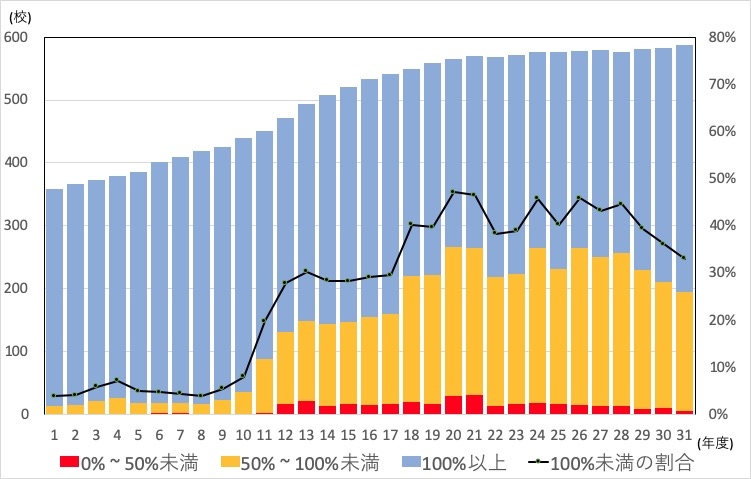
\includegraphics[scale=0.53]{images/shigansya.jpg}
\caption{平成元年〜31年の私立大学志願者数の推移}
\label{fig:shigan}
\end{figure}
大学数は増加傾向にあったものの,ここ10年間はほぼ横ばいである.
志願者数が募集人数を下回った大学の比率は近年減少傾向にある.これは2018年から大学に対して入学者の超過率を厳格に制限\cite{hojokin1}したためであると考えられる.
超過率の厳格化によって入学者数が絞られる形になり,その分の学生が他の大学に流れた結果,定員割れの大学数が減少した.
さらに平成31年からは入学定員充足率が 0.9 〜 1.0 倍の場合に入学定員充足率に応じて補助金が増額される\cite{hojokin2}.
そのため今後,有名大学の入学者数は減少した後に一定になると予想される.
この政策を政府が主導して施行した理由を論座の記事\cite{ronza}から引用する.
\begin{quotation}
「私立大学の入学定員管理の厳格化」(以下、定員厳格化)とは、大都市圏の大規模私立大学に学生が集中している状況を改善するため、文科省が2016年度から始めた政策である。

私立大学の予算には国から交付される助成金が含まれており、その額は大学にもよるが、平均して大学の年間収入額の1割前後にもなる。
定員厳格化は、所定の枠を超えて入学させる大学に対してその助成金を交付しないという、いわば「金で大学を縛る」政策なのである。
\end{quotation}
また論座の記事には,このような定員厳格化の影響で,不本意入学による学生と大学のミスマッチが起こる可能性について論じている.

さらにこの状況を示したデータとして,所属大学の選択理由に関する私立大学学生生活白書2018\cite{reason}のアンケート結果を図 \ref{fig:reason}に示す.
「自宅からの通学が可能だったから」,「自分の力に合っていたから」,「他に合格した大学がなかったから」,「大都市にあるから」,などが理由として多く回答されていることがわかる.
\begin{figure}[H]
\centering
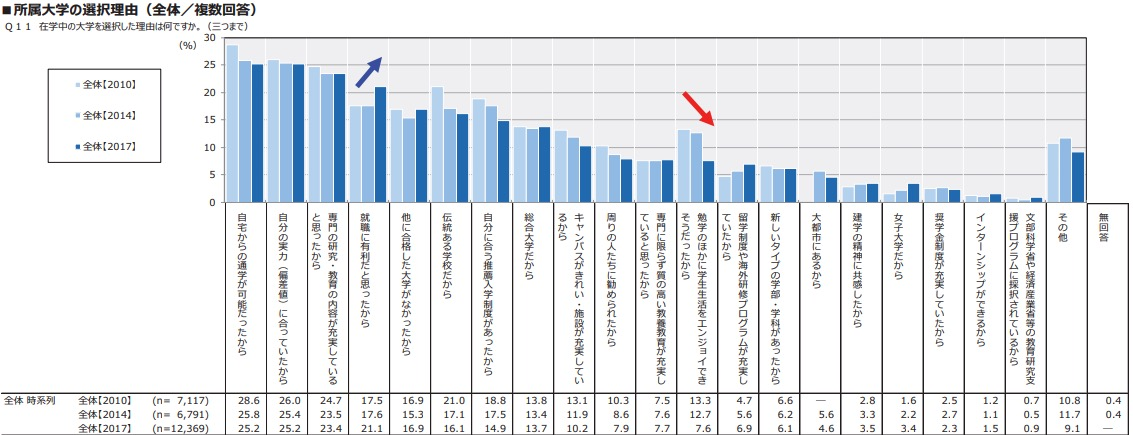
\includegraphics[width=20cm, angle=90]{images/SS.jpg}
\caption[所属大学選択理由]{所属大学選択理由 \cite{reason}}
\label{fig:reason}
\end{figure}
本来の意味を考えれば,講義内容や力を入れている研究分野,校風などを加味して,自分に合った大学を選ぶべきである.
しかし実際には,安定思考や偏差値,立地といった尺度だけで大学を選択する傾向にある.

このような傾向においては,大学定員厳格化の効果は限定的と言わざるを得ない.
定員が守られることが周知されることによって,合格の見込みのない生徒は単により偏差値の低い大学の受験にシフトしただけである.
定員割れの対策にはなっているが,大学選びの本質からはずれている.

本質的な問題点は,大学を選ぶ際の基準が画一化している点である.
そのため大都市の大学,有名大学等に志願者が集中する事態に陥っている.
この問題を解決するためには,大学選択において,1つの尺度で大学を選択するのではく,総合的な観点から関係性を持った大学を提示し,自分にあった大学を選ぶ必要がある.


\section{研究目的}
本研究の大きな目的は,大学を選ぶ際の基準となる情報を提示するシステムを構築することである.
基準となる情報提示を実現するためには,各大学の特徴や大学同士の潜在的な関連性や共通性などの知識表現を蓄えることが必要である.
また,それらの情報を引き出し,提示する可視化システムが必要となる.
以上の目的を実現するため,具体的には大学に関する記事から単語ベクトルを学習し,偏差値やキャンパス所在地などの情報を補助的に利用して,大学間の関係性を可視化するための支援をするシステムを構築する.

\section{関連研究}
大学名を単語ベクトルで表現して,潜在的な関係性を可視化するという点で,関連した研究は存在しなかった.
単語ベクトル同士で単語の比較をする点においては,明畠ら\cite{thesis1}の研究で,Word2Vecを用いた趣味嗜好の類似度計算をコサイン類似度を用いておこなっている.
本研究においても,大学同士の単語ベクトルの類似度計算にはコサイン類似度を用いた.

\section{論文構成}
2章では本研究で使用した詳細な技術について説明する.
3章では変研究で提案するシステムの説明と実際に構築したシステムの使用方法を解説する.
4章ではシステムの有効性を検証した結果についてまとめる.
最後に5章で有効性の考察を考察し,本研究のまとめと今後の課題について述べる.